\documentclass[conference]{IEEEtran}
\usepackage{cite}
\usepackage{amsmath,amssymb,amsfonts}
\usepackage{algorithmic}
\usepackage{graphicx}
\usepackage{textcomp}
\usepackage{xcolor}
\usepackage{hyperref}
\usepackage{tabularx}

% COMMANDS
\newcommand{\R}{\mathbb{R}}
\newcommand{\fig}[1]{\textit{Figure \ref{1}}}
\newcommand{\eq}[1]{\textit{Equation \ref{1}}}

\begin{document}

\title{Applied AI in Biomedicine - Workshop Report}

% AUTHORS
\author{
Alberto Rota
\IEEEauthorblockA{ \\
\textit{Person Code: 10615751}\\
\textit{Student Number: 964662} \\
\href{mailto:alberto2.rota@mail.polimi.it}{alberto2.rota@mail.polimi.it}}\\
\and
Gabriele Santicchi 
\IEEEauthorblockA{ \\
\textit{Person Code: 10579046}\\
\textit{Student Number: 969088}  \\
\href{mailto:gabriele.santicchi@mail.polimi.it}{gabriele.santicchi@mail.polimi.it}}
}
\maketitle

\section{Introduction}
\subsection{Dataset}

\section{Data Preprocessing}
The available raw dataset undergoes a pre-processing phase necessary for the
optimal interfacing between the data and the model.
\subsection{Exploratory Data Analysis}

\subsection{Signal Windowing}
The heartbeat-by-heartbeat classification that the model performs implies the
necessity of splitting the 30 minutes recording of each patient in windows, each
one to be processed separately by the network:
choosing the proper width and the optimal windowing approach is key in
obtaining the best model performance. Three different approaches have been taken
into consideration when splitting the windows, which are graphically compared in
\fig{fig:windows}.
\begin{figure}
    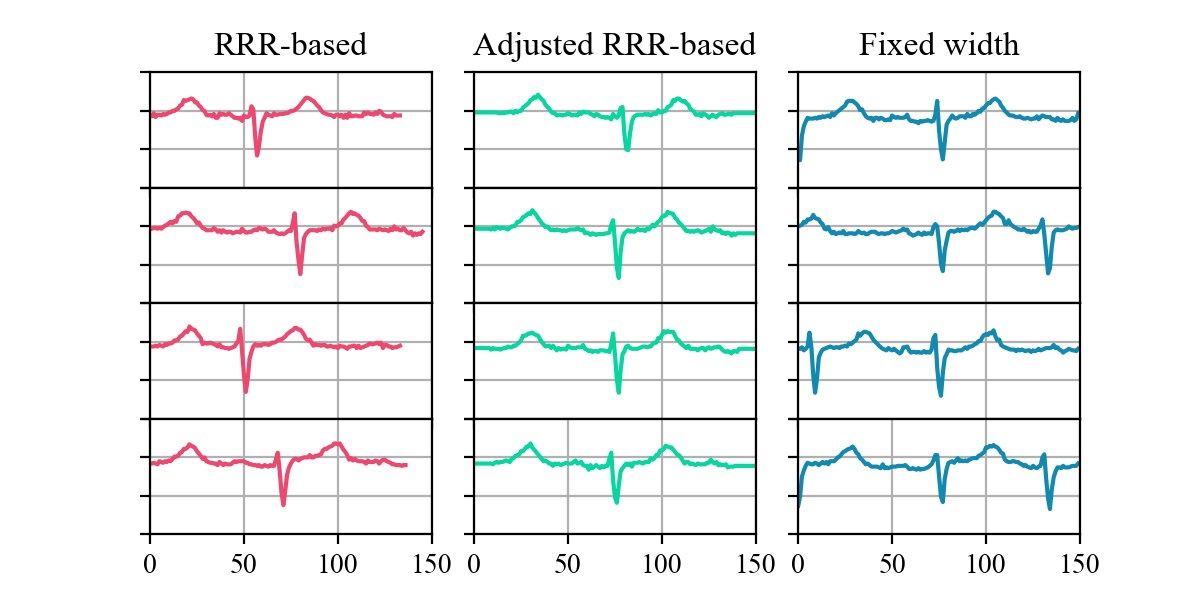
\includegraphics[width=\linewidth]{img/windowing.png}
    \label{fig:windows}
\end{figure}



\subsection{Class imbalance}

\section{Implementation}

\section{Results}

\section{Discussion}

\section{Conclusions}

\end{document}